\documentclass[a4paper,12pt]{article}
\usepackage{amsmath,amssymb,amsthm} 
% for x'
\usepackage{mathtools,textcomp}
\usepackage{url}
\usepackage{hyperref}
\usepackage[left=20mm,top=20mm]{geometry}

\usepackage{fontspec}
 % Times New Roman
% \setmainfont[Path = fonts/, 
% BoldFont=TimesNewerRoman-Italic.otf,
% ItalicFont=TimesNewerRoman-Italic.otf,
% BoldItalicFont=TimesNewerRoman-BoldItalic.otf
% ]{TimesNewerRoman-Regular.otf}

% 中文字
\usepackage{xeCJK}
\setCJKmainfont[Path = fonts/ , AutoFakeBold=true,AutoFakeSlant=true]{cwTeXKai.ttf}
\XeTeXlinebreaklocale "zh"
\XeTeXlinebreakskip = 0pt plus 1pt
\setlength{\parskip}{0.3cm}

\usepackage{xcolor}
\newcommand{\alert}[1]{\textcolor{red}{\textbf{#1}}}

% make hyperlink reference with color
\usepackage{hyperref}
\hypersetup{
    colorlinks=true,
    linkcolor=blue
}

% sub title
\newcommand{\subtitle}[1]{\Large{#1}}

% multiple reference
\usepackage{cleveref}

% pandoc .md to .tex
\providecommand{\tightlist}{%
  \setlength{\itemsep}{0pt}\setlength{\parskip}{0pt}}

\title{HOMEWORK ASSIGNMENT \#3 \\ \subtitle{Morphological Processing, Texture Analysis}}
\author{Poy Lu 呂栢頤 \\ D09944015 \\ 網媒所博一 \\ \url{ariapoy@gmail.com}}

\date{\today}

% no paragraph indent overall document
\setlength\parindent{0pt}
\begin{document}

\maketitle

%\section{Problem 1: WARM-UP}\label{problem-1-warm-up}
Original image \cref{fig1} for question \textbf{(a)} \& \textbf{(b)}.
\begin{figure}
    \centering
    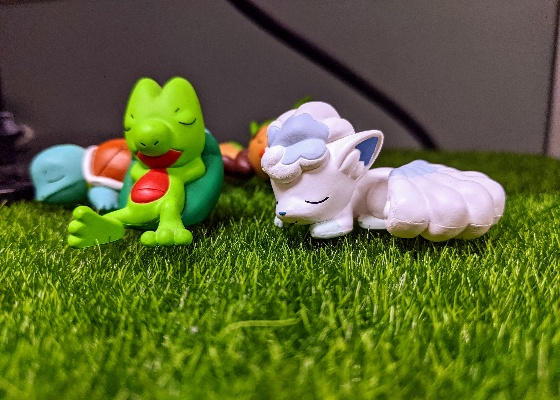
\includegraphics[width=0.7\textwidth]{image/sample1.jpg}
    \caption{\textbf{sample1.jpg}}
    \label{fig1}
\end{figure}

\textbf{(a)} Convert the given color image, \textbf{sample1.jpg}, to a grayscale image named \textbf{1\_result.jpg}.

\textbf{Motivation}
Be familiar with \texttt{Pillow (PIL)} \& \texttt{NumPy}.

\textbf{Approach}
Define \texttt{rgb2gray} function \(\mbox{Grayscale} = 0.2989 * r + 0.5870 * g + 0.1140 * b\) with following \href{https://stackoverflow.com/questions/12201577/how-can-i-convert-an-rgb-image-into-grayscale-in-python}{Stackoverflow reference}.

Note: The coefficient is designed that the human eye is most sensitive to the intensity region. We could also adjust them to get different results.

\textbf{Performance of results}
Result of problem 1(a): \textbf{1\_result.jpg} \cref{fig1a}.
\begin{figure}
    \centering
    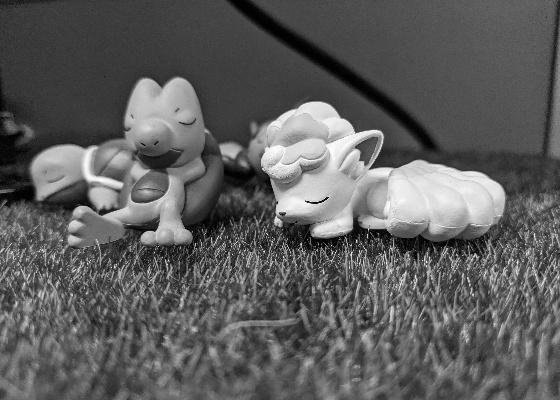
\includegraphics[width=0.7\textwidth]{image/1_result.jpg}
    \caption{\textbf{1\_result.jpg} Colorful to grayscale}
    \label{fig1a}
\end{figure}

\textbf{Discussion}
It looks good. ;-)


\textbf{(b)} Perform horizontal flipping on \textbf{sample1.jpg} and output the result as \textbf{2\_result.jpg}.

\textbf{Motivation}
Be familiar with \texttt{Pillow (PIL)} \& \texttt{NumPy}.

\textbf{Approach} 
Reverse the order of \textbf{column} a.k.a \textbf{second axis} of image array.

\textbf{Performance of results}
Result of problem 1(b): \cref{fig1b}.
\begin{figure}
    \centering
    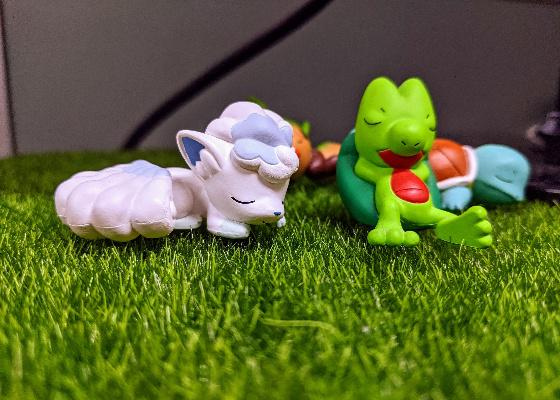
\includegraphics[width=0.7\textwidth]{image/2_result.jpg}
    \caption{\textbf{2\_result.jpg} Horizontal flipping}
    \label{fig1b}
\end{figure}

\textbf{Discussion}
It looks good. ;-)

%\newpage
\section{Problem 2: FREQUENCY DOMAIN}\label{problem-2-frequency-domain}
In this problem, please perform Fourier transform and observe the relation between the spatial domain and the frequency spectrum. You may adopt tools for Fourier transform. The recommended tools are listed in the Appendix.

Original image \nameref{sample2} for question \nameref{2_a} \nameref{2_b}, \nameref{2_c}.
\begin{figure}
    \centering
    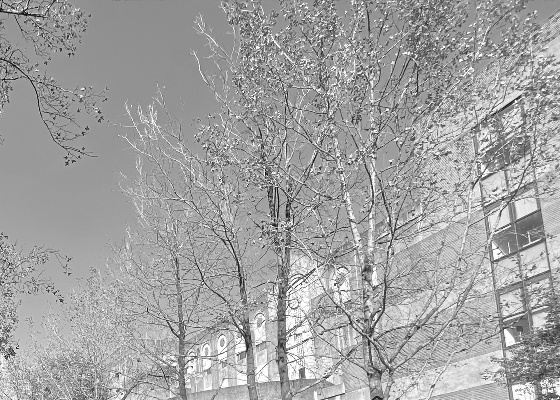
\includegraphics[width=0.7\textwidth]{src/sample2.png}
    \caption{\textbf{sample2.jpg}}
    \label{sample2}
\end{figure}

\subsection{(a)}\label{2_a}
Perform Fourier transform on \textbf{sample2.png} to obtain its frequency spectrum and output it as \textbf{result5.png}. (Please take the log magnitude of the absolute value and center the low frequency part at the origin for visualization.)

\paragraph{Motivation}

\paragraph{Approach}

\paragraph{Performance of results}
In the end, I choose the \alert{settings}...

Result of problem 2(a): \nameref{result5}.
\begin{figure}
    \centering
    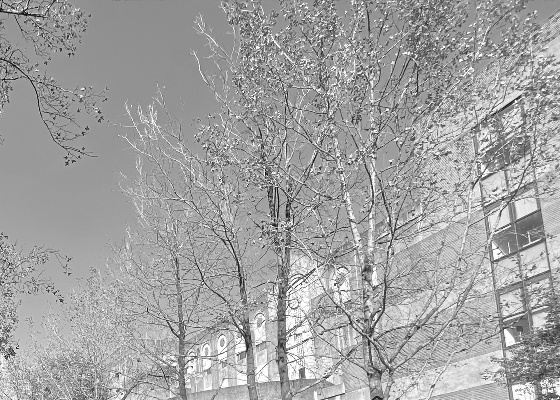
\includegraphics[width=0.7\textwidth]{src/sample2.png}
    \caption{\textbf{result5.jpg} Log axis of frequency domain}
    \label{result5}
\end{figure}

\paragraph{Discussion}

\subsection{(b)}\label{2_b}
Based on the result of part (a), design and apply a low-pass filter in the frequency domain and transform the result back to the pixel domain by inverse Fourier transform. The resultant image is saved as \textbf{result6.png}. Please also design a low-pass filter in the pixel domain which behaves similarly to the one you design in the frequency domain. Output the result as \textbf{result7.png} and provide some discussions.

\paragraph{Motivation}

\paragraph{Approach}

\paragraph{Performance of results}
In the end, I choose the \alert{settings}...

Result of problem 2(b): \nameref{result6}.
\begin{figure}
    \centering
    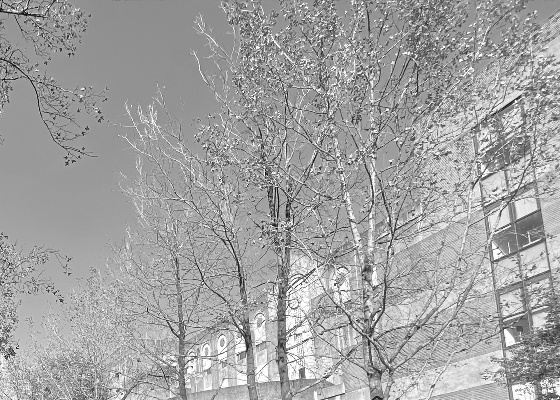
\includegraphics[width=0.7\textwidth]{src/sample2.png}
    \caption{\textbf{result6.jpg} Low-pass filter in frequency domain}
    \label{result6}
\end{figure}

Result of problem 2(b): \nameref{result7}.
\begin{figure}
    \centering
    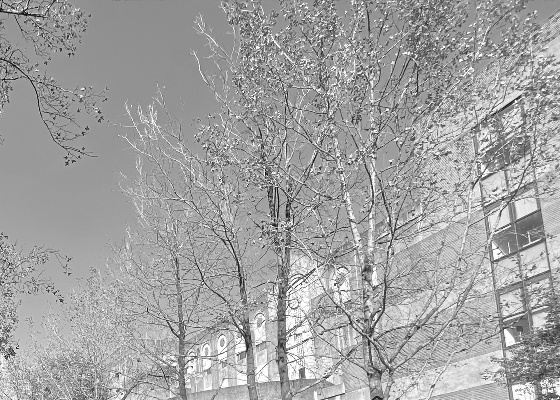
\includegraphics[width=0.7\textwidth]{src/sample2.png}
    \caption{\textbf{result7.jpg} Low-pass filter in spatial domain}
    \label{result7}
\end{figure}

\paragraph{Discussion}
Compare \nameref{result6} with \nameref{result7}.

\subsection{(c)}\label{2_c}
Based on the result of part (a), design and apply a high-pass filter in the frequency domain and transform the result back to the pixel domain by inverse Fourier transform. The resultant image is saved as \textbf{result8.png}. Please also design a high-pass filter in the pixel domain which behaves similarly to the one you design in the frequency domain. Output the result as \textbf{result9.png} and provide some discussions.

\paragraph{Motivation}

\paragraph{Approach}

\paragraph{Performance of results}
In the end, I choose the \alert{settings}...

Result of problem 2(c): \nameref{result8}.
\begin{figure}
    \centering
    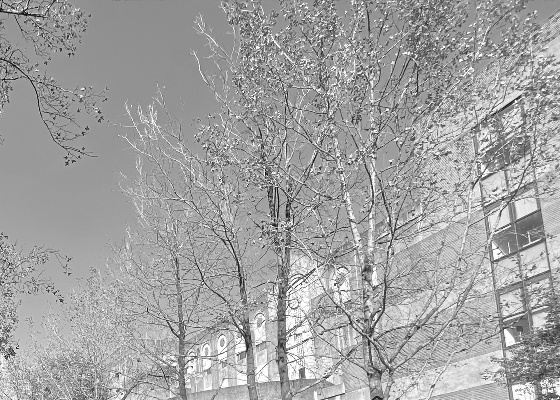
\includegraphics[width=0.7\textwidth]{src/sample2.png}
    \caption{\textbf{result8.jpg} High-pass filter in frequency domain}
    \label{result8}
\end{figure}

Result of problem 2(c): \nameref{result9}.
\begin{figure}
    \centering
    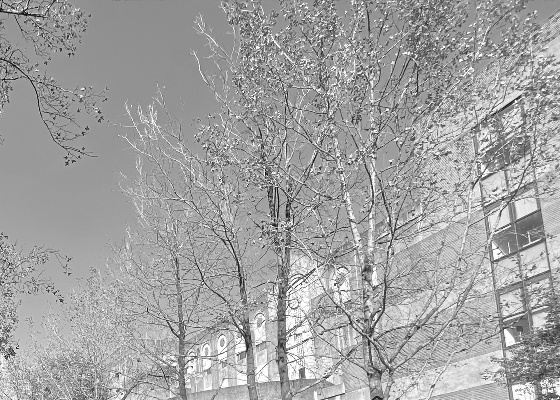
\includegraphics[width=0.7\textwidth]{src/sample2.png}
    \caption{\textbf{result7.jpg} High-pass filter in spatial domain}
    \label{result9}
\end{figure}

\paragraph{Discussion}
Compare \nameref{result8} with \nameref{result9}.

Original image \nameref{sample3} for question \nameref{2_d} \nameref{2_e}.
\begin{figure}
    \centering
    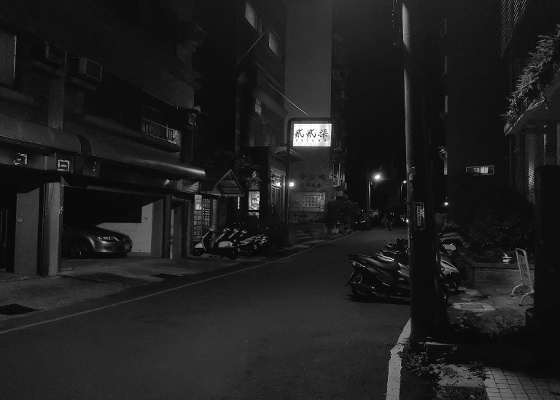
\includegraphics[width=0.7\textwidth]{src/sample3.png}
    \caption{\textbf{sample3.jpg}}
    \label{sample3}
\end{figure}

\subsection{(d)}\label{2_d}
Perform Fourier Transform on \textbf{sample3.png} and output it as \textbf{result10.png}. Please discuss what you observe in \textbf{sample3.png} and \textbf{result10.png}.

\paragraph{Motivation}

\paragraph{Approach}

\paragraph{Performance of results}
In the end, I choose the \alert{settings}...

Result of problem 2(d): \nameref{result10}.
\begin{figure}
    \centering
    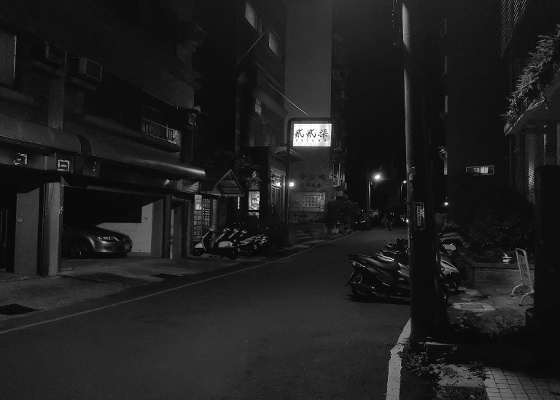
\includegraphics[width=0.7\textwidth]{src/sample3.png}
    \caption{\textbf{result10.jpg} Fourier Transform on \nameref{sample3}}
    \label{result10}
\end{figure}

\paragraph{Discussion}
Observe in \nameref{sample3} and \nameref{result10}.

\subsection{(e)}\label{2_e}
Try to remove the undesired pattern on \textbf{sample3.png} and output it as \textbf{result11.png}.

\paragraph{Motivation}

\paragraph{Approach}

\paragraph{Performance of results}
In the end, I choose the \alert{settings}...

Result of problem 2(e): \nameref{result11}.
\begin{figure}
    \centering
    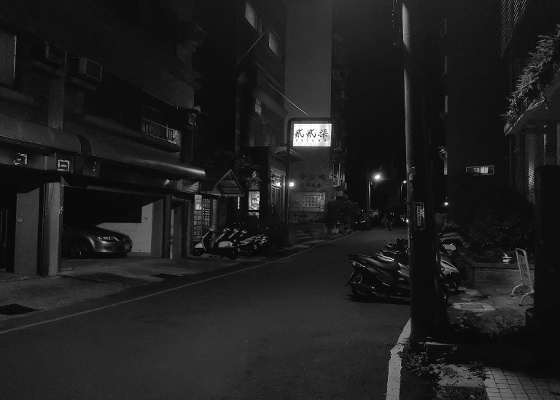
\includegraphics[width=0.7\textwidth]{src/sample3.png}
    \caption{\textbf{result11.jpg} Noise cleaning of \nameref{sample3}}
    \label{result11}
\end{figure}

\paragraph{Discussion}


\end{document}
